\documentclass{TIJMUjiaoanSY}
\pagestyle{empty}


\begin{document}


%课程名称
\kecheng{Linux系统概论}
%实验名称
\shiyan{实验7\ Vim编辑器的基本操作}
%教师姓名
\jiaoshi{伊现富}
%职称
\zhicheng{讲师}
%教学日期(格式:XXXX年XX月XX日XX时-XX时)
\riqi{2015年6月25日15:30-17:30}
%授课对象(格式:XXX系XXXX年级XX班(硕/本/专科))
\duixiang{生物医学工程学院2013级生信班(本)}
%实验人数
\renshu{28}
%实验类型
\leixing{验证型}
%实验分组
\fenzu{一人一机}
%学时数
\xueshi{2}
%教材版本
\jiaocai{Linux系统概论上机指南(自编教材)}


%教案首页
\firstHeader
\maketitle
\thispagestyle{empty}

\mudi{
\begin{itemize}
  \item 掌握Vim的主要工作模式及模式间的转换方法。
  \item 掌握Vim的基本操作:新建保存、移动定位、修改删除、复制粘贴、重做撤消和查找替换等。
\end{itemize}
}

\fenpei{
\begin{itemize}
  \item (10')工作模式:回顾Vim的主要工作模式,总结进行模式转换的方法。
  \item (10')基本操作:回顾总结Vim中新建保存、移动定位、修改删除、复制粘贴、重做撤消和查找替换等基本操作的常用命令。
  \item (80')实验操作:练习Vim的基本操作,掌握Vim的使用方法。
\end{itemize}
}

\cailiao{
\begin{itemize}
  \item 主要仪器:一台安装有Vim编辑器的计算机。
\end{itemize}
}

\zhongdian{
\begin{itemize}
  \item 重点难点:Vim的主要模式及模式转换,移动定位和编辑的基本命令。
  \item 解决策略:通过实例进行讲解,通过演示进行学习,通过练习熟练掌握。
\end{itemize}
}

\sikao{
\begin{itemize}
  \item Vim的工作模式主要有哪三种?
  \item 在Vim中如何进行模式的转换?
  \item Vim中最基本的移动命令是哪四个?
  \item 进入Vim输入模式的命令有哪些?
  \item 在Vim中如何进行剪切、复制和粘贴?
  \item 在Vim中如何进行撤销和重做?
  \item 在Vim中如何进行搜索和替换?
  \item 启动、保存文件和退出Vim的命令有哪些?
\end{itemize}
}

\cankao{
\begin{itemize}
  \item Linux基础及应用习题解析与实验指导(第二版),谢蓉\ 编著。中国铁道出版社,2014。
\end{itemize}
}

\firstTail


%教案续页
\newpage
\otherHeader

\noindent
\begin{enumerate}
  \item 工作模式(10分钟)
    \begin{itemize}
\parpic[fr]{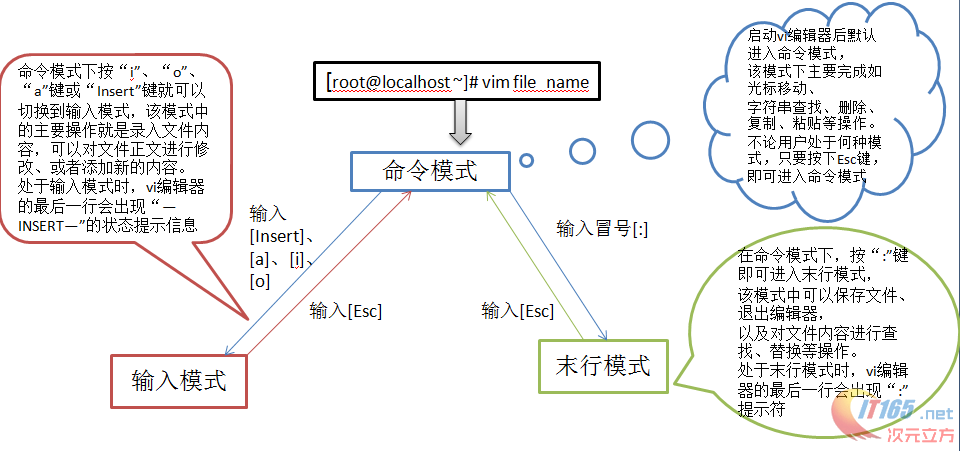
\includegraphics[width=9cm,height=5cm]{c7.vim.mode.01.png}}
      \item 命令模式:Vim启动后的默认模式,所有输入都被解释成命令
      \item 输入模式:大部分按键都会向缓冲区中插入文本
      \item 末行模式:可以输入会被解释并执行的文本
      \item 可视模式:使用移动命令高亮选择字符、行或文本块
      \item 替换模式:每个输入的字符都会覆盖文本缓冲区中存在的字符
    \end{itemize}

  \item 基本操作(10分钟)
    \vspace*{-10pt}
    \begin{multicols}{2}
      \begin{enumerate}
	\item 基本移动:h,j,k,l
	\item 移动定位:0,\verb|^|,\verb|$|,w,b,gg,G
	\item 进入输入模式:i,I,a,A,o,O
	\item 剪切删除:x,X,d,D,dd
	\item 修改替换:cc,r,R,s,S
	\item 复制粘贴:J,yy,Y,p,P
	\item 撤销重做:u,U,Ctrl+R
	\item 搜索替换:/word,?word,s/old/new/
	\item 保存退出::q,:w,:wq,:q!,:x,ZZ
      \end{enumerate}
    \end{multicols}
    \vspace*{-10pt}
    \begin{figure}[h]
      \centering
      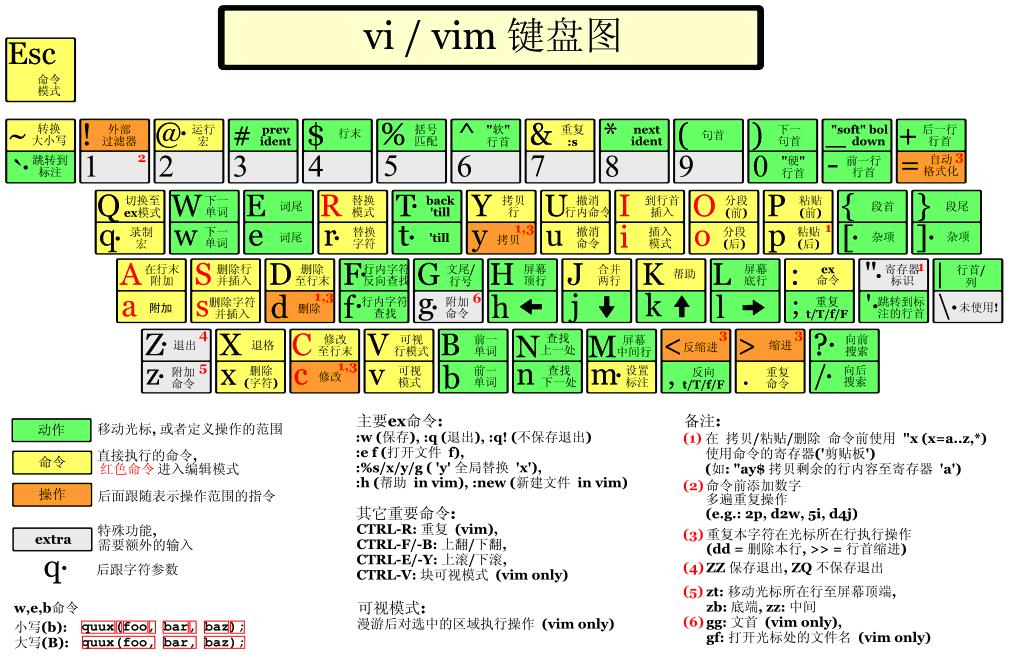
\includegraphics[width=17cm]{c7.vim.shortcut.06.jpg}
    \end{figure}
    \vspace*{-10pt}

  \item 实验操作(80分钟)
    \begin{enumerate}
      \item 新建文本文件\textcolor{red}{(基本命令:i,Esc,:w,:q)}
      \item 编辑文件\textcolor{red}{(基本命令::set nu,O,s,u,d,h,j,k,l)}
      \item 其他基本操作的常见命令\textcolor{red}{(启动,保存,退出,移动定位,修改删除,复制粘贴,搜索替换,等)}
    \end{enumerate}
\end{enumerate}

\otherTail


\end{document}

